\documentclass[12pt]{article}

\usepackage{booktabs}% http://ctan.org/pkg/booktabs
\usepackage[utf8]{inputenc}
\usepackage{changepage}
\usepackage{pgfplots}
\usepackage{amssymb}
\usepackage{xcolor}
\usepackage{hyperref}
\usepackage{listings}
\usepackage[T1]{fontenc}
\usepackage[utf8]{inputenc}
\usepackage{adjustbox}
\usepackage{amsmath}
\usepackage{mathtools}
\usepackage{biblatex}
\lstset{
  language=Python,
  numbers=left,
  numberstyle=\tiny,
  stepnumber=1,
  numbersep=5pt,
  tabsize=4,
  basicstyle=\ttfamily,
  columns=fullflexible,
  keepspaces,
}
\hypersetup{
    colorlinks,
    citecolor=black,
    filecolor=black,
    linkcolor=black,
    urlcolor=black
}

% Set page size and margins
% Replace `letterpaper' with `a4paper' for UK/EU standard size
\usepackage[letterpaper,top=2cm,bottom=2cm,left=3cm,right=3cm,marginparwidth=1.75cm]{geometry}

% Useful packages
\usepackage{amsmath}
\usepackage{mathtools}
\usepackage{graphicx}
\newenvironment{para}{\begin{adjustwidth}{13mm}{}}{\end{adjustwidth}}

\newcommand\tab[1][1cm]{\hspace*{#1}}

\newcommand{\tabitem}{\llap{\textbullet}}
\newcommand{\Hsquare}{%
\text{\fboxsep=-.2pt\fbox{\rule{0pt}{1ex}\rule{1ex}{0pt}}}%
}

\newtheorem{Definizione}{Definizione}[subsection]
\newtheorem{Lemma}{Lemma}[subsection]
\newtheorem{Teorema/Definizione}{Teorema/Definizione}[subsection]
\newtheorem{Corollario}{Corollario}[subsection]
\newtheorem{Teorema}{Teorema}[subsection]
\newtheorem{Proposizione}{Proposizione}[subsection]
\newtheorem{Notazione}{Notazione}[subsection]
\newtheorem{Commento}{Commento}[subsection]
\newtheorem{Dimostrazione}{Dimostrazione}[subsection]
\newtheorem{Osservazione}{Osservazione}[subsection]
\newtheorem{Nota}{Nota}[subsection]


\title{Analisi e Progettazione del Software}
\author{spitfire}
\date{A.A. 2023-2024}
\begin{document}
\begin{figure}
    \centering
    
\includegraphics[width=0.35\textwidth]{Images/Logo scienze bicocca.png}
\end{figure}

\vspace{10cm}
\date{A.A. 2023-2024}


\maketitle

\newpage

\tableofcontents
\newpage

\section{Introduzione}
Che cos'è il \textbf{software}? Esso è \textbf{un programma per computer} unito alla \textbf{documentazione ad esso associata},
la quale specifica e comprende \textbf{requisiti, modelli di progetto, manuale utente,...} \newline
I prodotti software possono essere:
\begin{itemize}
    \item \textbf{Generici}: sviluppati per un ampio insieme di clienti (elaboratori di testo, database,...)
    \item \textbf{Personalizzati} (custom): sviluppati per un singolo cliente in base alla sue esigenze specifiche
\end{itemize}
Un nuovo prodotto software può essere \textbf{creato da zero, personalizzando software già esistenti o riusando parti o software già esistente}.
Le caratteristiche essenziali di un buon software sono:
\begin{center}
    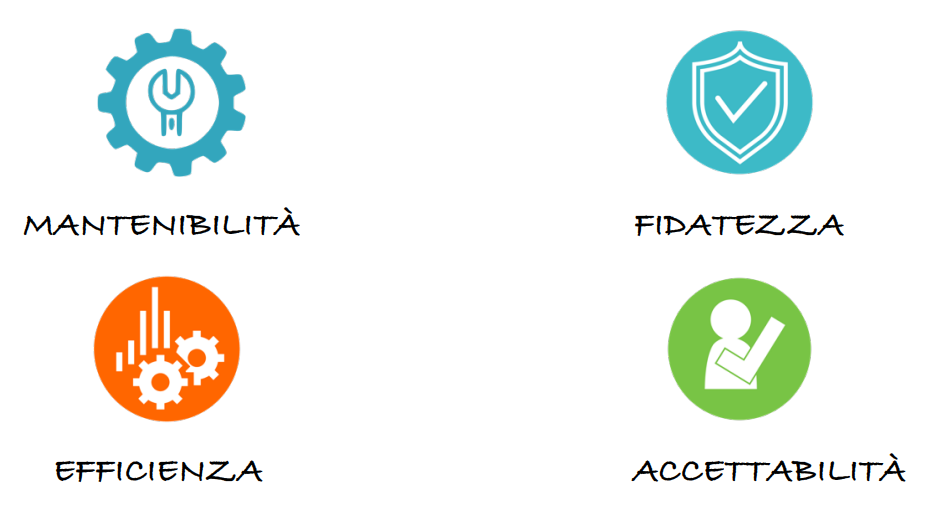
\includegraphics[width = 0.80\textwidth]{Images/1.png}
\end{center}
\subsection{Introduzione all'ingegneria del software}
Che cos'è \textbf{l'ingegneria del software}? \textbf{L'ingegneria del software} è una disciplina ingegneristica che si occupa
di tutti gli aspetti della produzione del software di buona qualità, dalle \textbf{prime fasi della specifica del sistema fino alla manutenzione del sistema}
dopo la messa in uso. Vediamo cosa si intende per \textbf{disciplina ingegneristica} e "\textbf{Tutti gli aspetti della produzione del software}":
\begin{itemize}
    \item \textbf{Disciplina ingegneristica}: Utilizzare metodi e teorie \textbf{appropriati} per risolvere i problemi tenendo conto dei vincoli \textbf{organizzativi e finanziari}
    \item \textbf{Tutti gli aspetti della produzione del software}: Non solo il \textbf{processo tecnico di sviluppo}. Anche la \textbf{gestione del progetto} e lo sviluppo di \textbf{strumenti}
    ,metodi ecc... per supportare la produzione del software
\end{itemize}
\newpage
\noindent
La disciplina dell'ingegneria del software si occupa di:
\begin{center}
    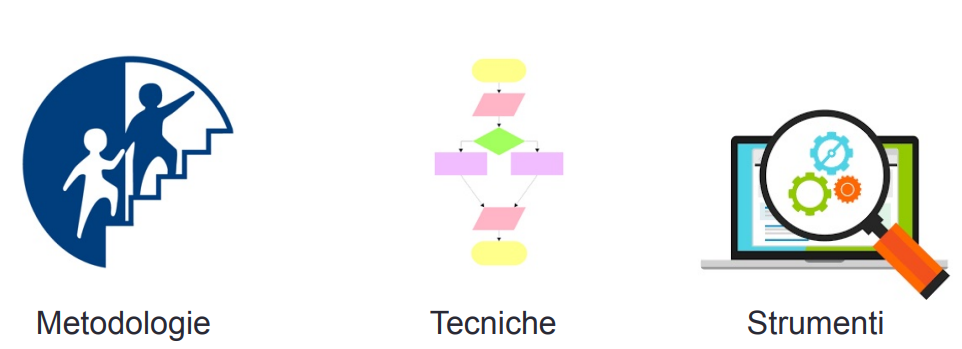
\includegraphics[width = 0.80\textwidth]{Images/2.png}
\end{center}
\subsection{La crisi del software}
Il termine \textbf{crisi del software} (o software crisis) è usato nell'ambito dell'ingegneria del software per descrivere l'impatto della \textbf{rapida crescita} della potenza degli elaboratori
e la \textbf{complessità} dei problemi che dovevano esseri affrontati. Le parole chiavi della software crisis erano \textbf{complessità, attese e cambiamento}. Il concetto di software crisis emerse negli
anni '60.
\begin{center}
    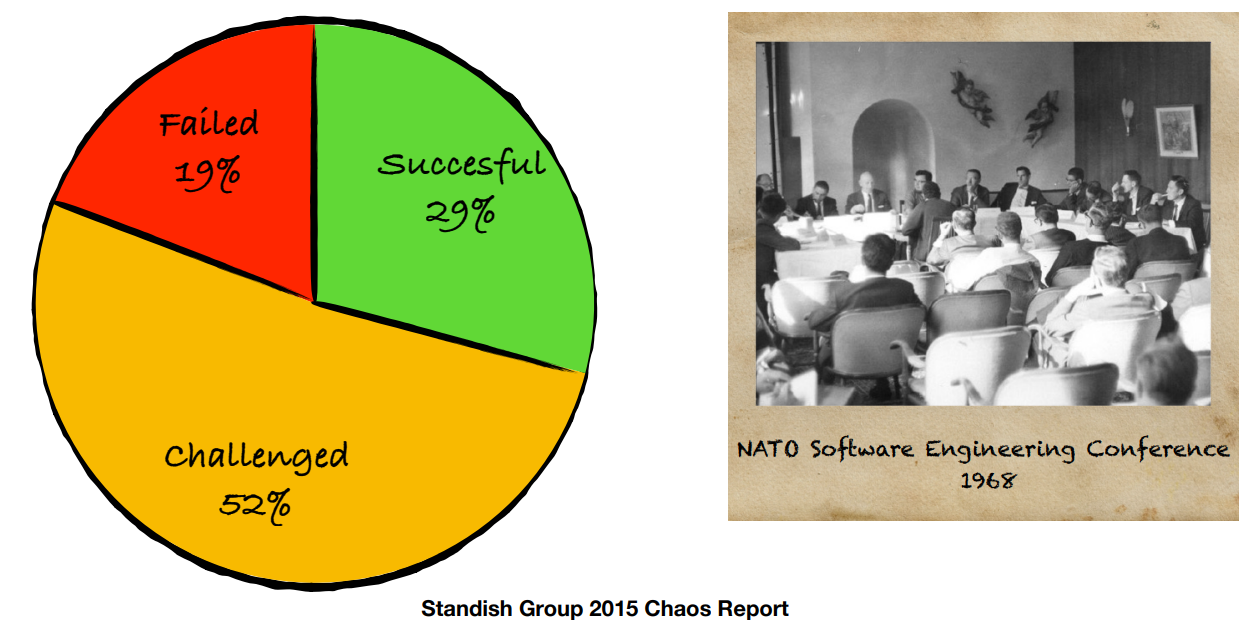
\includegraphics[width = 0.80\textwidth]{Images/3.png}
\end{center}
\begin{center}
    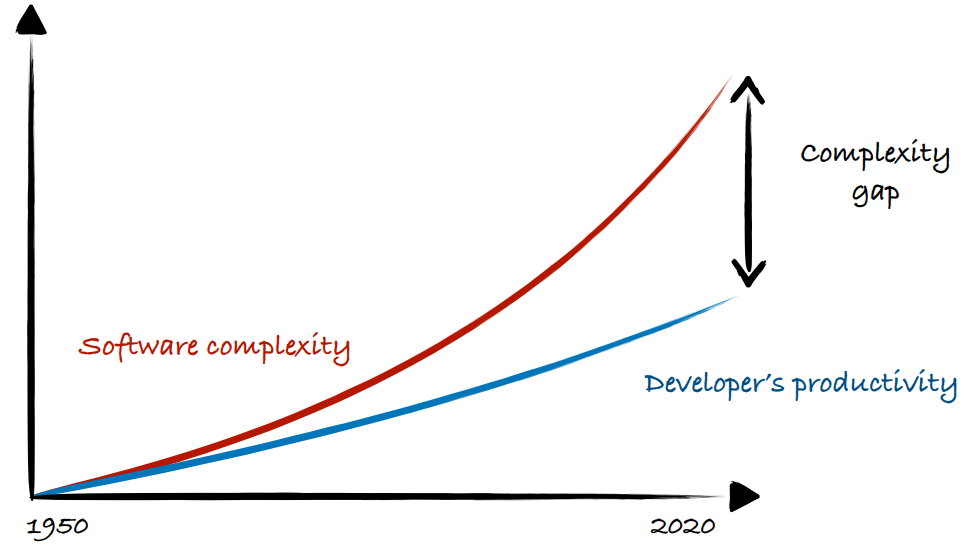
\includegraphics[width = 0.80\textwidth]{Images/4.png}
\end{center}
Le cause della crisi del software erano legate alla \textbf{complessità dei processi software} e alla \textbf{relativa immaturità dell'ingegneria del software}
Per superare la crisi infatti si dovettero introdurre:
\begin{itemize}
    \item \textbf{Management}
    \item \textbf{Organizzazione}, attraverso \textbf{analisi e progettazione}
    \item \textbf{Teorie e tecniche} come la \textbf{programmazione strutturata e ad oggetti}
    \item \textbf{Strumenti}, come gli IDE
    \item \textbf{Metodologie}, tra cui il \textbf{modello a cascata e il modello agile}
\end{itemize}
\subsection{Analisi e progettazione}
Che cosa sono \textbf{analisi e progettazione}? \newline
\textbf{L'analisi} enfatizza un'\textbf{investigazione del problema e dei requisiti} invece che una soluzione: per esempio, se si vuole realizzare un nuovo sistema di trading online,
bisognerà capire \textbf{come questo sistema verrà utilizzato} e \textbf{quali sono le sue funzioni}. "Analisi" è un termine ampio con più accezioni, tra cui:
\begin{itemize}
    \item \textbf{Analisi dei requisiti}, cioè un'investigazione dei requisiti del sistema
    \item \textbf{Analisi orientata agli oggetti}, cioè un'investigazione degli oggetti di dominio
\end{itemize} 
La \textbf{progettazione} enfatizza una soluzione \textbf{concettuale} (software e hardware) che \textbf{soddisfa i requisiti}, anziché la relativa implementazione. Per esempio, la descrizione di uno schema di base di dati
e di oggetti software. Nella progettazione vengono spesso \textbf{esclusi dettagli di basso livello o "ovvi"} (o almeno "ovvi" per coloro a cui è destinato il software). \newline
Infine i progetti possono essere \textbf{implementati} e la loro implementazione (ovvero il codice) esprime il progetto realizzato vero e completo.
Come nel caso dell'analisi, anche "progettazione" è un termine con più accezioni, tra cui:
\begin{itemize}
    \item \textbf{Progettazione orientata agli oggetti}
    \item \textbf{Progettazione di basi di dati}
\end{itemize}
L'analisi e la progettazione possono essere riassunti con la seguente frase:
\begin{center}
    \textbf{Fare la cosa giusta}(analisi) \textbf{e fare la cosa bene}(progettazione)
\end{center}
\subsubsection{Analisi e progettazione orientata agli oggetti}
Durante \textbf{l'analisi orientata agli oggetti} c'è un enfasi sull'\textbf{identificazione} e la \textbf{descrizione degli oggetti}, o dei \textbf{concetti}, nel \textbf{dominio del problema}.
Per esempio, nel caso di un sistema informatico per voli aerei, alcuni dei concetti possono essere \textit{Aereo, Volo} e \textit{Pilota}. \newline
Durante \textbf{la progettazione orientata agli oggetti} (o più semplicemente \textbf{progettazione a oggetti}) l'enfasi è sulla \textbf{definizione di oggetti software} e sul \textbf{modo in cui questi collaborano
per soddisfare i requisiti}. Per esempio un oggetto software \textit{Aereo} può avere un attributo \textit{codiceDiRegistrazione} e un metodo \textit{getVoliEffettuati}. \newline
\begin{center}
    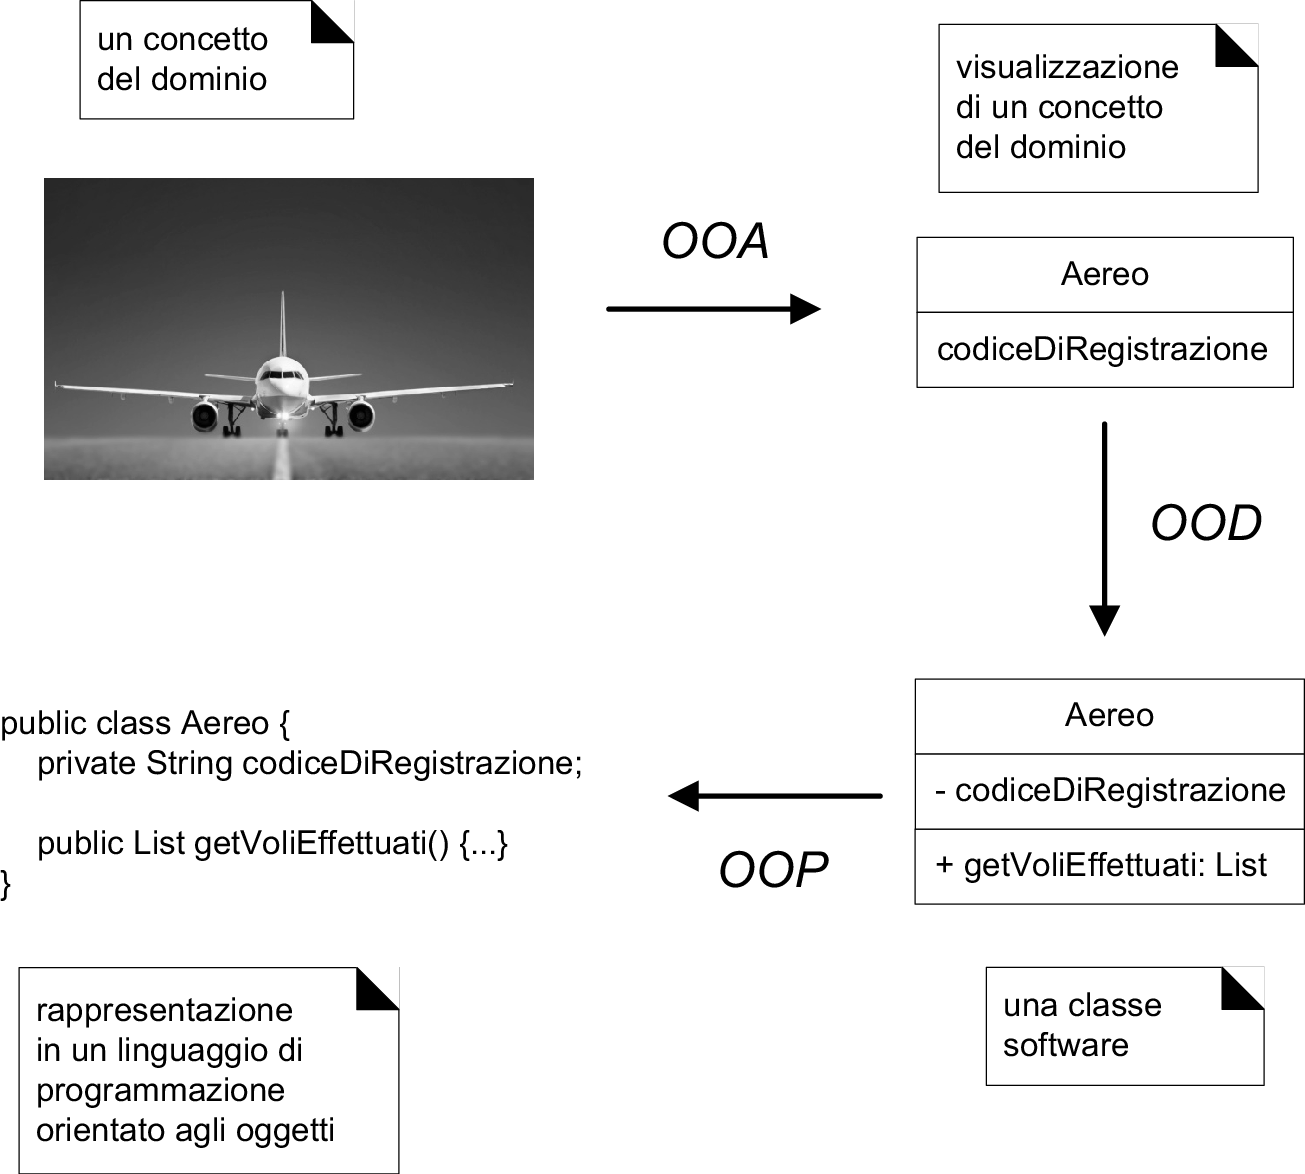
\includegraphics[width = 0.70\textwidth]{Images/5.png}
\end{center}
Infine durante \textbf{l'implementazione} o la \textbf{programmazione orientata agli oggetti}, gli oggetti progettati vengono implementati, per esempio implementando la classe \textit{Aereo} in un linguaggio ad oggetti.
Dunque, analisi e progettazione \textbf{hanno obbiettivi diversi che vengono perseguiti in maniera diversa}. Tuttavia, come mostrato dall'esempio sopra, esse sono \textbf{attività fortemente sinergiche} che sono \textbf{correlate fra loro}
e con le \textbf{altre attività dello sviluppo del software}.
\subsection{Introduzione ai diagrammi e ai passi fondamentali dello sviluppo software}
Vediamo una breve introduzione dei \textbf{vai diagrammi e dei passi fondamentali} legati allo sviluppo software.
\begin{center}
    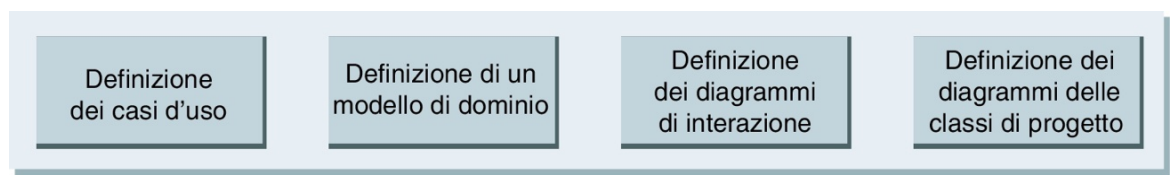
\includegraphics[width = 0.80\textwidth]{Images/6.png}
\end{center}
\subsubsection{Definizione dei casi d'uso}

\textbf{L'analisi dei requisiti} può comprendere \textbf{storie o scenari} relativi al modo in cui l'applicazione può essere utilizzata dagli utenti;
queste storie possono essere scritte come \textbf{casi d'uso}. I casi d'uso \textbf{non sono un elaborato ad oggetti} ma semplicemente delle storie scritte. Sono tuttavia
uno strumento \textbf{diffuso nell'analisi dei requisiti}. Facciamo un'esempio: \newline
\textbf{Gioca una partita a Dadi}: Il giocatore chiede di lanciare i dadi. Il Sistema presenta il risultato: se il valore totale delle facce dei dadi è sette, il giocatore ha vinto; altrimenti ha perso.
\subsubsection{Definizione di un modello di dominio}
L'analisi orientata agli oggetti è interessata alla \textbf{creazione di una descrizione del dominio da un punto di vista ad oggetti}. Vengono identificati i \textbf{concetti, gli attributi e le associazioni considerati significativi}.
Il risultato può essere espresso come un \textbf{modello di dominio} che mostra i concetti o gli oggetti \textbf{significativi} del dominio. Esso è rappresentato nel seguente modo:
\begin{center}
    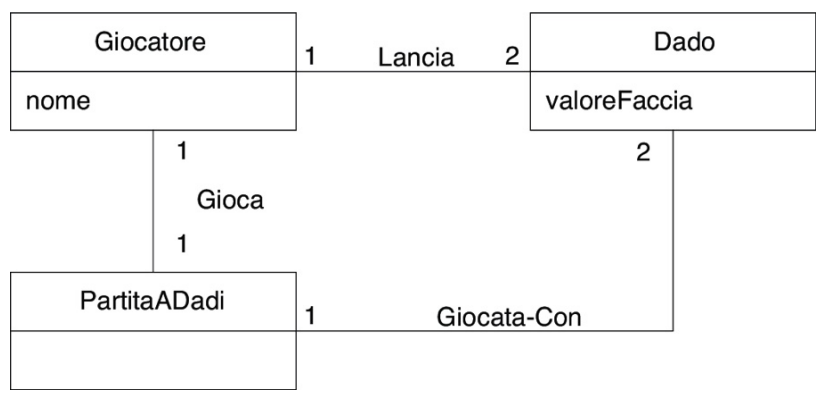
\includegraphics[width = 0.65\textwidth]{Images/7.png}
\end{center}
\subsubsection{Definizione dei diagrammi di interazione}
La \textbf{progettazione ad oggetti} è interessata alla \textbf{definizione di oggetti software, delle loro responsabilità e collaborazioni}. Una notazione comune per illustrare queste collaborazione è un
\textbf{diagramma di sequenza} (un tipo di diagramma UML). Esso mostra lo scambio di messaggi \textbf{tra oggetti software}, dunque l'invocazione di \textbf{metodi}. Esso è rappresentato nel seguente modo:
\begin{center}
    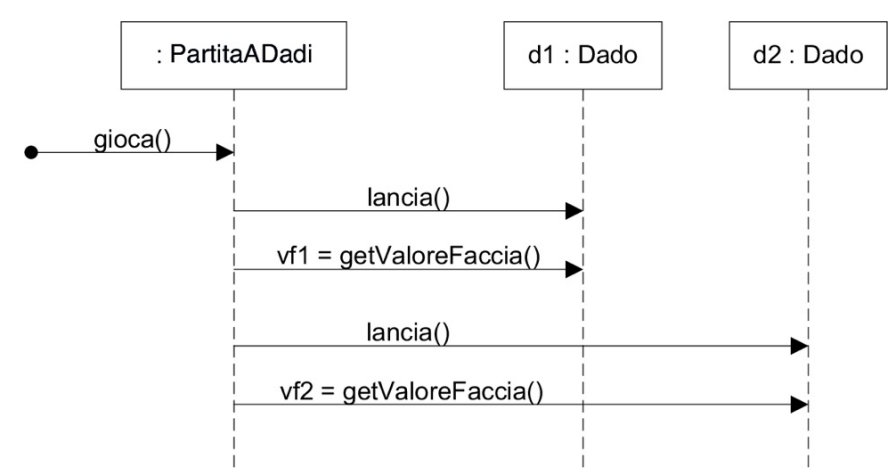
\includegraphics[width = 0.65\textwidth]{Images/8.png}
\end{center}
È interessante notare come \textbf{la progettazione degli oggetti software e dei programmi si può ispirare a un dominio del mondo reale}, tuttavia essa non è \textbf{nè un modello diretto nè una simulazione di questo dominio}. Quindi, per esempio,
seppur nel mondo reale è il giocatore a lanciare il dado, nel progetto software è l'oggetto \textit{PartitaADadi} che "lancia" i dadi.
\subsubsection{Definizione dei diagrammi di classe di progetto}
Accanto a una visione dinamica delle \textbf{collaborazioni tra oggetti}, mostrata dai diagrammi di interazione, è utile mostrare una \textbf{vista statica} delle definizioni di classi mediante un \textbf{diagramma delle classi di progetto}, che mostra le classi software 
con i loro attributi e metodi. Il diagramma delle classi di progetto è rappresentato nella seguente maniera:
\begin{center}
    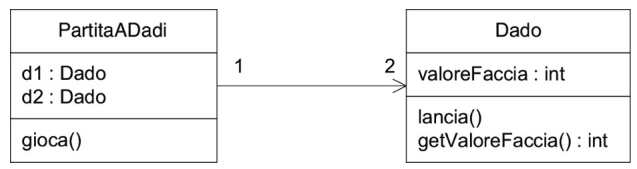
\includegraphics[width = 0.65\textwidth]{Images/9.png}
\end{center}
Diversamente dal modello di dominio, che illustra \textbf{classi del mondo reale}, questo diagramma mostra \textbf{classi software}.
Si noti che, benché questo diagramma delle classi di progetto \textbf{non sia uguale al modello di dominio}, i nomi e il contenuto delle classi sono \textbf{simili}. In tal modo i \textbf{progetti e i linguaggi Object Oriented} (OO) sono in grado di \textbf{favorire un salto rappresentazionale basso}
tra i componenti software e il nostro modello mentale di un dominio, \textbf{migliorando la comprensione}.
\subsection{UML}
\textbf{Unified Modelling Language}, abbreviato \textbf{UML}, è un \textbf{linguaggio visuale} per la \textbf{specifica, la costruzione e la documentazione degli elaborati} di un sistema software.
UML rappresenta una \textbf{collezione di best practices di ingegneria}, dimostratesi vincenti nella modellazione di sistemi vasti e complessi; inoltre esso \textbf{favorisce la divulgazione delle informazioni nella comunità dell'ingegneria del software} in quanto è \textit{standard de facto}.
Bisogna però tenere a mente che \textbf{UML non è una metodologia ma un linguaggio!} \newline
Il termine \textit{visuale} della definizione è un punto fondamentale. UML è uno standard de facto per la \textbf{notazione di diagrammi per disegnare o rappresentare figure} (con del testo) \textbf{relative al software}, e in particolare, al software OO.
A un livello più profondo, di particolare interesse per i produttori di strumenti per \textbf{MDA} (Model Driven Architecture) alla base della notazione UML c'è il \textbf{meta-modello di UML} che descrive la \textbf{semantica} degli elementi di modellazione, tuttavia non è necessario che lo sviluppatore lo conosca. 
Presentiamo ora una breve storia di UML:
\begin{center}
    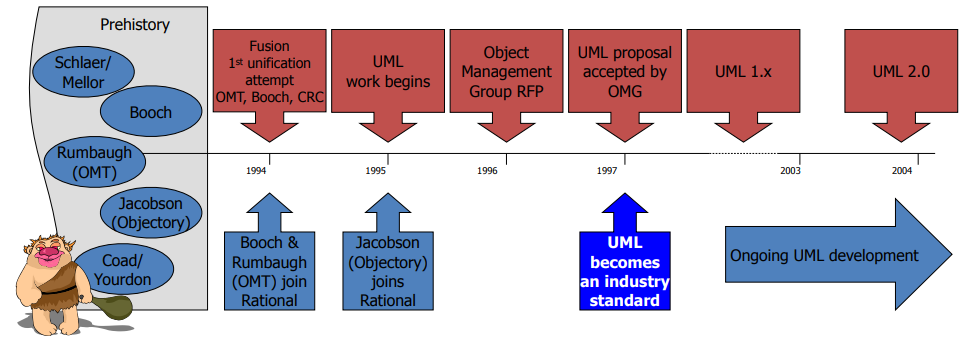
\includegraphics[width = 1.05\textwidth]{Images/10.PNG}
\end{center}
Il più significativo aggiornamento di UML è avvenuto nel \textbf{2003}:
\begin{itemize}
    \item Maggiore \textbf{consistenza}
    \item Semantica definita in maniera \textbf{più chiara e dettagliata}
    \item \textbf{Nuovi diagrammi}
    \item Compatibilità con le precedenti versioni (1.x)
\end{itemize}
Altra parola importante è \textit{unified}: UML vuole essere un \textbf{linguaggio unificante} sotto diversi aspetti:
\begin{itemize}
    \item \textbf{Storico} (OMT, Booch, CRC, Objectory)
    \item \textbf{Ciclo di sviluppo} (sintassi visuali per tutte le fasi)
    \item \textbf{Domini applicativi} (dai sistemi embedded ai sistemi gestionali)
    \item \textbf{Linguaggi e piattaforme di sviluppo} (.Net, Java, C\#,...)
    \item \textbf{Processi di sviluppo} (UP, BPM, ...)
\end{itemize}
\subsubsection{UML e gli oggetti}
UML modella i sistemi come \textbf{una serie di oggetti che collaborano fra loro}. Si hanno quindi due strutture:
\begin{itemize}
    \item \textbf{Struttura statica}:
    \begin{itemize}
        \item \textbf{Quali} tipi di oggetti sono necessari
        \item \textbf{Come} sono correlati
    \end{itemize}
    \item \textbf{Struttura dinamica}:
    \begin{itemize}
        \item \textbf{Ciclo di vita} di questi oggetti
        \item \textbf{Come collaborano} per fornire le funzionalità richieste
    \end{itemize}
\end{itemize}
\subsubsection{Tre modi di applicare UML}
\textbf{Fowler} [Fowler03] descrive tre modi per applicare UML:
\begin{itemize}
    \item \textbf{UML come abbozzo}: Diagrammi \textbf{informali e incompleti} (spesso abbozzati a mano su una lavagna bianca), che vengono creati per 
    \textbf{esplorare parti difficili dello spazio del problema o della soluzione}, sfruttando l'espressività dei linguaggi visuali.
    \item \textbf{UML come progetto}: Diagrammi di progetto abbastanza dettagliati che vengono utilizzati per:
    \begin{enumerate}
        \item \textbf{Il reverse engineering}, ovvero per visualizzare e comprendere meglio \textbf{del codice già esistente} mediante dei diagrammi UML. In questo caso, uno strumento UML legge il codice
        sorgente o binario per \textbf{generare} (di solito) \textbf{dei diagrammi UML dei package, delle classi e di sequenza}. Questi "progetti" possono aiutare il lettore a capire i principali elementi, le strutture e le collaborazioni
        \item \textbf{Il forward engineering}, ovvero per la \textbf{generazione di codice}. In questo caso, alcuni diagrammi dettagliati possono fornire una \textbf{guida alla generazione di codice} da fare manualmente o automaticamente con un strumento.
        Solitamente, i diagrammi sono utilizzati per \textbf{specificare una parte di codice}, mentre il resto del codice viene scritto da uno sviluppatore durante la codifica, magari applicando UML come abbozzo.
    \end{enumerate}
    \item \textbf{UML come linguaggio di programmazione}: La specifica \textbf{completamente eseguibile} di un sistema software con UML.
    Il codice viene generato \textbf{automaticamente} e non viene normalmente normalmente né visto né modificato dagli sviluppatori; quindi UML viene usato come vero e proprio \textbf{linguaggio di programmazione}.
    Questo utilizzo di UML richiede un modo \textbf{pratico} per rappresentare sotto forma di di diagrammi \textbf{tutto il comportamento o la logica} (probabilmente tramite diagrammi di interazione e di stato).
    Si tratta di un approccio \textbf{ancora in corso di sviluppo} sia in termini di teoria sia in termini di usabilità e robustezza degli strumenti.
\end{itemize}
La \textbf{modellazione agile} enfatizza l'uso di UML come \textbf{abbozzo}; si tratta di un metodo comune per applicare UML, spesso con un elevato ritorno in termini di \textbf{investimento di tempo} (che è normalmente breve).
\subsubsection{Due punti di vista per applicare UML}
UML descrive dei tipi \textbf{grezzi} di diagrammi, come i diagrammi delle classi e i diagrammi di sequenza; tuttavia UML \textbf{non impone un particolare punto di vista di modellazione per l'uso di questi diagrammi}; 
quindi la stessa notazione può essere usata secondo \textbf{due punti di vista} (o prospettive) e \textbf{tipi di modelli}:
\begin{itemize}
    \item \textbf{Punto di vista concettuale}: I diagrammi sono scritti e interpretati \textbf{come descrizioni di oggetti del mondo reale} o nel dominio di interesse
    \item \textbf{Punto di vista software}: I diagrammi, che utilizzano \textbf{la stessa notazione del punto di vista concettuale}, descrivono astrazioni o componenti software. In particolare, i diagrammi possono descrivere:
    \begin{enumerate}
        \item \textbf{Implementazioni software} con riferimento a una particolare tecnologia
        \item \textbf{Specifiche e interfacce} di componenti software, ma \textbf{indipendentemente} da ogni possible implementazione
    \end{enumerate}
\end{itemize}
\begin{center}
    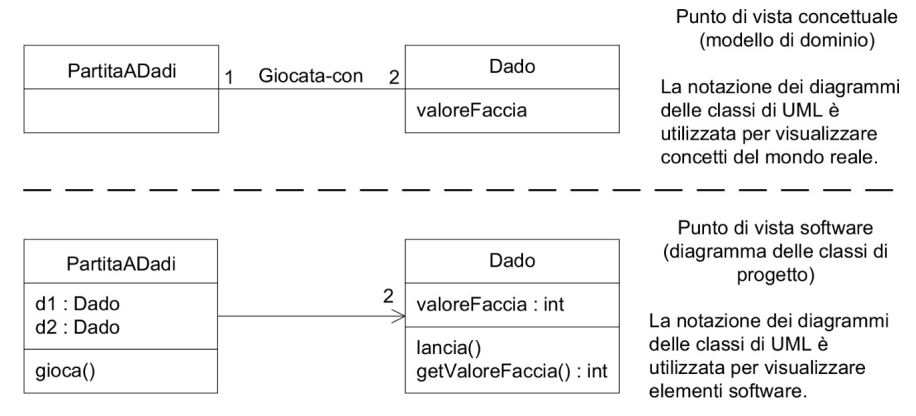
\includegraphics[width = 0.80\textwidth]{Images/11.PNG}
\end{center}
Quindi, in pratica, UMl viene usato:
\begin{enumerate}
    \item \textbf{Nell'analisi}, principalmente secondo il \textbf{punto di vista concettuale}
    \item \textbf{Nella progettazione}, principalmente secondo il \textbf{punto di vista software}
\end{enumerate}
\subsubsection{Significato di classe}
Nell'UML grezzo, abbiamo chiamato "classi" un insieme di oggetti; ma questo termine racchiude una \textbf{varietà di casi}: oggetti fisici, concetti astratti, elementi software, eventi e così via.
In particolare, una classe UML è un caso particolare di un modello UML generale chiamato \textbf{classificatore}, che è qualcosa che ha delle caratteristiche strutturali e/o comportamentali e comprende \textbf{classi, attori, interfacce e casi d'uso}.
Un metodo \textbf{impone una terminologia alternativa sovrapposta all'UML grezzo}; in particolare, ci adegueremo a quella di \textbf{UP} (Unified Process), che chiama:
\begin{itemize}
    \item \textbf{Classe concettuale}: Oggetto o concetto \textbf{del mondo reale} da un punto di vista \textbf{concettuale}. Il modello di dominio di UP contiene \textbf{classi concettuali}
    \item \textbf{Classi software}: Una classe che rappresenta un \textbf{componente software}, da un punto di vista \textbf{software}, indipendentemente dal processo, metodo o linguaggio di programmazione. Il modello di progetto di UP contiene \textbf{classi software}.
\end{itemize}
\subsubsection{Vantaggi della modellazione visuale}
Disegnare e leggere UML implica che si sta lavorando in \textbf{modo visuale}. La modellazione visuale ci permette di sfruttare le capacità del nostro cervello di \textbf{comprendere rapidamente simboli, unità e relazioni nelle notazioni} (prevalentemente bidimensionali) a "rettangoli e linee".
I diagrammi ci aiutano a vedere o esaminare meglio il \textbf{quadro generale} e le relazione tra elementi dell'analisi del software e allo stesso tempo ci permettono di \textbf{ignorare o nascondere i dettagli poco interessanti}.
\section{Processi per lo sviluppo del software}
Un \textbf{processo per lo sviluppo del software} (o \textbf{processo software}) definisce un approccio disciplinato per la \textbf{costruzione}, il \textbf{rilascio} e la \textbf{manutenzione del software}.
Definisce quindi \textbf{chi fa che cosa, quando e come} per raggiungere un certo obbiettivo. In particolare:
\begin{itemize}
    \item \textbf{Cosa} sono le \textbf{attività}
    \item \textbf{Chi} sono i \textbf{ruoli}
    \item \textbf{Come} sono le \textbf{metodologie}
    \item \textbf{Quando} riguarda \textbf{l'organizzazione temporale} delle attività
\end{itemize} 
\newpage
\noindent
Le attività fondamentali di un processo di sviluppo sono:
\begin{center}
    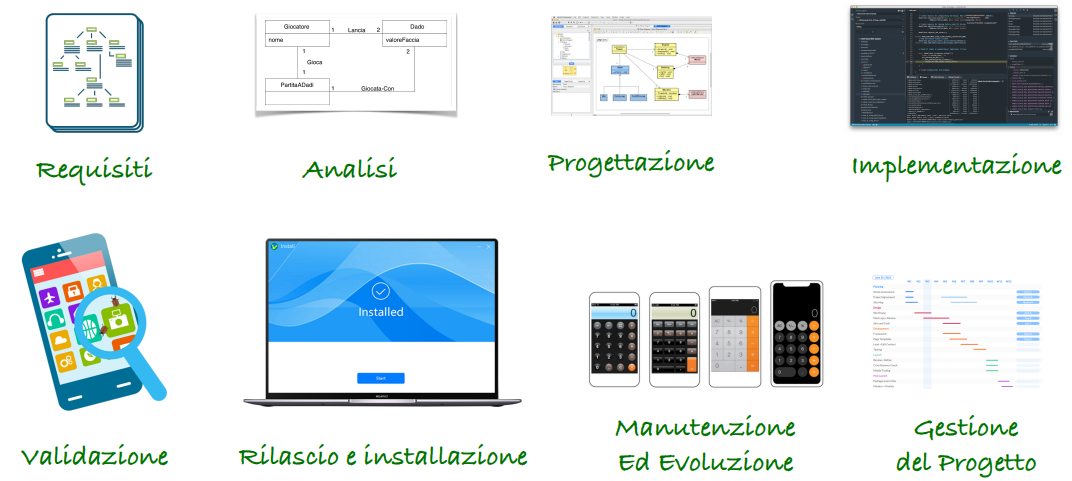
\includegraphics[width = 1\textwidth]{Images/12.PNG}
\end{center}

\end{document}
